\documentclass{article}

\usepackage{siunitx} % Provides the \SI{}{} and \si{} command for typesetting SI units

\usepackage{graphicx} % Required for the inclusion of images

\usepackage{tabularx} % Tables

\usepackage{natbib} % Required to change bibliography style to APA
\usepackage{float}
\usepackage{hyperref}
\usepackage[normalem]{ulem}
\useunder{\uline}{\ul}{}

\usepackage{amsmath} % Required for some math elements

% Many options for pseudocode
\usepackage{algorithm2e}
\usepackage{algorithmic}

\usepackage{listings} % Python code blocks
\usepackage[margin=1in]{geometry} % CUSTOM

\setlength\parindent{0pt} % Removes all indentation from paragraphs

\title{Lab 6 Report: Path Planning and Following with Simultaneous Localization} % Title

\author{Team 22 \\\\ Benjamin Rich \\ Dinuri Rupasinghe \\ Sophia Wang \\ Steven Liu \\ Jose Soto  \\ Editor for Lab 6: Sophia Wang\\\\ 16.405/6.4200} % Team # + Names, Class (RSS)

\date{\today} % Date for the report
\begin{document}

\maketitle


\tableofcontents
\newpage


\section{Introduction (Author: Steven Liu)}

The purpose of this lab is to build on previous labs by having the robot now generate a plan on its own and be able to autonomously execute that plan. Specifically, the racecar should be able to navigate on its own between an arbitrary start and end point in a known environment, the Stata basement. This is a natural extension of the subjects covered in lab 5. While localization on its own can be useful, it falls short of full autonomy. Navigation is one of the simpler planning tasks, but one that has clear real-world applications, such as self-driving cars or autonomous factory robots that have to move from place to place efficiently and safely. \\

We are specified to utilize ROS software given by the course staff of Robotics, Science, and Systems. We will be utilizing the LiDAR sensor data we receive from the racecar, odometry data from the wheels and steering, the racecar router for transferring this data, and built-in ROS packages to implement the Python scripts we will be creating. \\

The goal of this lab is to successfully implement algorithms for path planning and path following in order for the racecar to successfully navigate between any two points of the State basement. This explicitly builds on lab 5: the code for Monte Carlo Localization runs in parallel with the new code, since the racecar has to know where it is in the first place in order to navigate. \\

We tackle the technical problem in several steps. Specific algorithms are chosen for the two parts, specifically A* search for the path planning and pure pursuit for trajectory following, chosen for their relative simplicity and sufficient performance in practice. These can be evaluated separately, both qualitatively by observing their behavior in simulation and quantitatively using the autograder provided by course staff. Once good performance is achieved in simulation, they along with the localization code are deployed to the racecar, where further tuning occurs. Tests of the integrated system can likewise be evaluated qualitatively through observation. In addition, performance is measured quantitatively by observing the cross-track error as the racecar navigates the trajectory.

\section{Technical Approach (Author: Benjamin Rich)}


\subsection{Overview}
As explained in the introduction, for this lab we have three primary technical goals: 
\begin{enumerate}
    \item Given a map, a goal, and a start position, generate a collision-free path from the start to the goal position. 
    \item Given a path in the form of a list of points, follow this path with the racecar as closely as possible.
    \item Incorporate (1) and (2) in real-time using localization to figure out the location of the car relative to the path, thus enabling path planning and simultaneous path following and localization. 
\end{enumerate}
We tackled these three goals in roughly sequential order; first demonstrating path planning abilities, then figuring out how to follow these paths, and lastly incorporating the prior capabilities on the physical racecar, along with our localization method from Lab 5. Figure 1, shown below, helps to demonstrate how these technical checkpoints work together to enable the car to plan and follow a path. 

\textbf{\begin{figure}[H]
\begin{center}
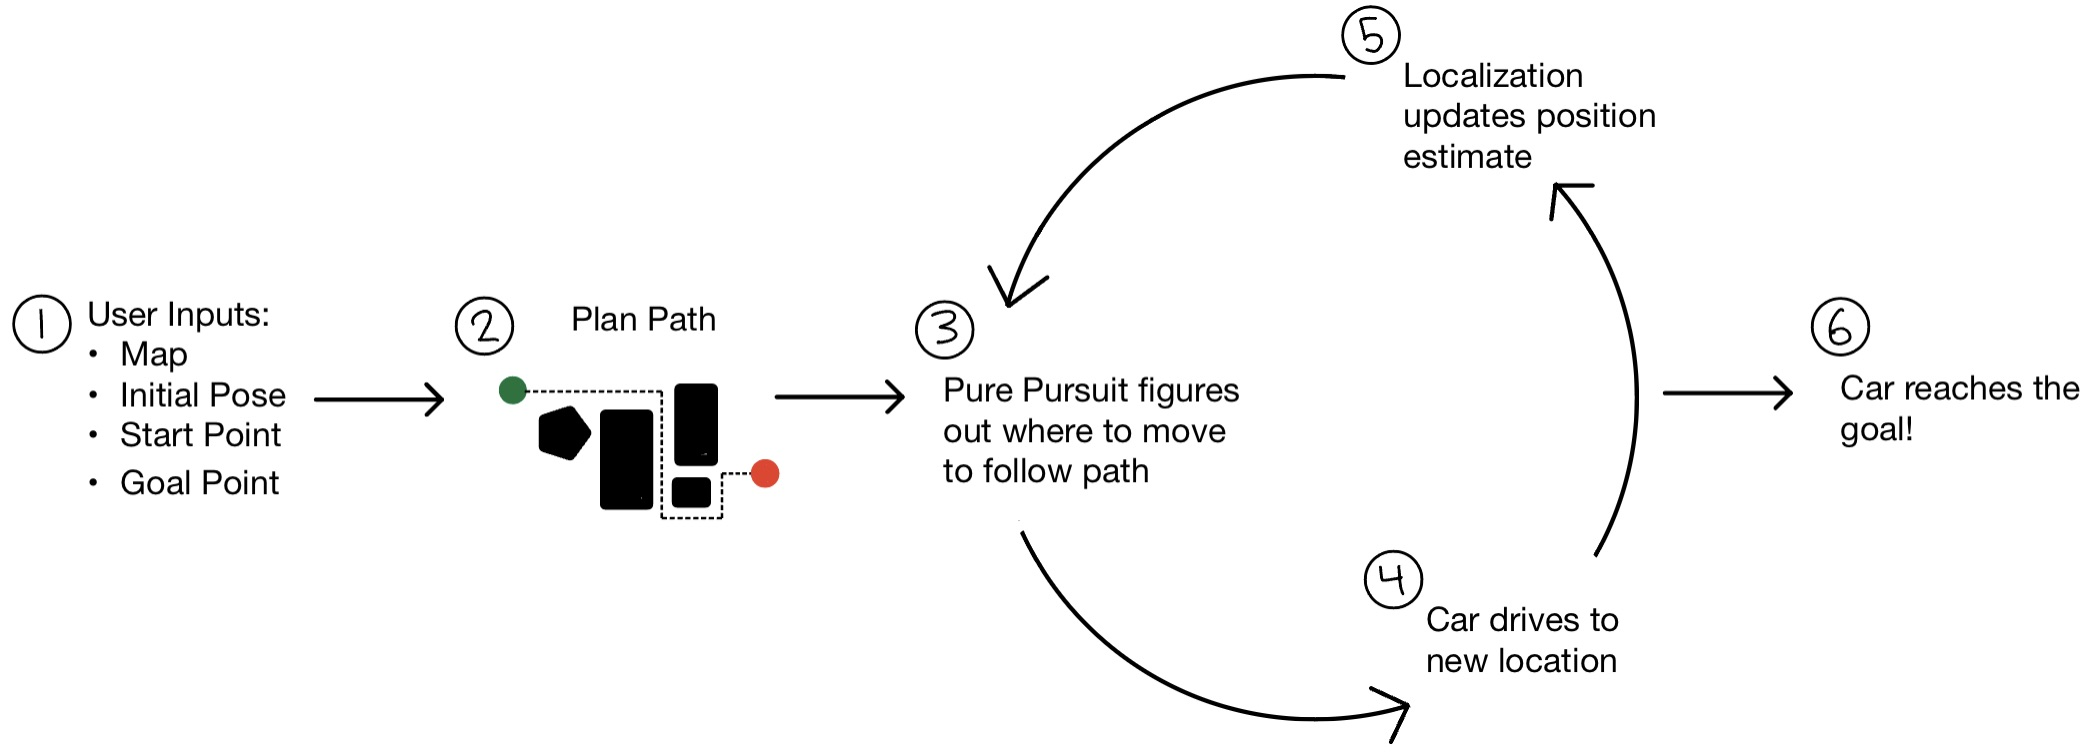
\includegraphics[width=0.85\textwidth]{process.png} % 
\caption{Visualization of Path Planning and Following Processs}
\end{center}
\label{workflow}
\end{figure}}



\subsection{Path Planning}
Path planning is the process of creating a path with some characteristics from one position to another. Usually, this path tries to maximize or minimize some property, such as reward, distance, time-taken to drive along the path, cost of the path, etc. Path planning has huge applications in an incredibly wide set of fields, including city construction, driving, autonomous mobilization, robotics, etc. In many case, what may not immediately be seen as a path-planning problem can be eventually solved using path-planning methods. For example, the act of moving a multi-jointed robot arm so that it can pick something up is actually a path-planning problem; we have to determine when and where to move the joints! Additionally, an incredible amount of computer science problems (graph search) are solved in the same way as some path planning problems. In short; path planning is incredibly interesting and has direct applications to numerous fields. \\

In the case of our car, we want to plan a path such that we minimize the time it takes to drive along the path while avoiding obstacles and ensuring the path is followable with a physical racecar (i.e. we can't do 90-degree point turns very well).  

\subsubsection{Types of Path Planning Algorithms}
Path planning algorithms come in all shapes and sizes, but can be classified into two main categories; graph-based algorithms which plan a path by dividing space into a discrete graph, and sample-based algorithms which plan a path by sampling continuous space. \\


\textbf{\underline{Graph-Based Path Planning Algorithms}}\\[1mm]
Graph-based algorithms work by dividing space into a graph. A graph, defined by $G=(V,E)$, is a structure defined by vertices ($v\in V$) and edges $(e\in E)$ which connect two vertices and may have weight and direction. Given a graph, graph-based planning algorithms explore the graph until they find a path to the goal. Graph-Based planning algorithms and numerous and have wide applications. Below is a short list of some common graph-based path planning algorithms, and a short description of how they operate: 
\begin{itemize}
    \item \textbf{Breadth-First Search (BFS)}: BFS is a general search algorithm that explores the next path in a LIFO (Last In First out) queue. Thus, BFS explores all paths of equal number of edges from the start position before exploring a path with a greater number of edges from the start position. BFS is guaranteed to find a path with the shortest number of edges from the start to goal when operating on a finite graph, but is not well suited to handling edge weights. Finite positive edge weights can be handled by edge expansion (i.e. for an edge of weight 3 create 2 nodes inside the edge for a total of 3 edges) but this increases runtime and cannot handle large magnitude edge weights. BFS has an asymptotic runtime of $O(|V|+|E|)$ and thus has linear runtime in the size of the graph. 
    \item \textbf{Depth-First Search (DFS)}: DFS is a general search algorithm very similar to BFS, except that it explores a chosen path as far as possible before being forced to backtrack. Thus, while DFS is guaranteed to find a path to a goal if one exists, it is not guaranteed to be the shortest. DFS also has linear asymptotic runtime of $O(|V|+|E|)$. 
    \item \textbf{Dijkstra's Algorithm}: Dijkstra's algorithm is a general search algorithm that handles positive weight edges, and thus is often well-suited for path planning. Dijkstra's explores paths in order of increasing distance from the start point, and continually updates a set of minimum distances to each node in the graph using edge relaxation (the concept that if $d[a]>d[b]+w_{edge:b,a}$ then we should update $d[a]=d[b]+w_{edge:b,a}$). Dijkstra's is guaranteed to find the shortest path of a weighted graph as long as all weights are positive or zero. With a fibonacci heap acting as the queue, Dijkstra's has asymptotic runtime of $O(|V|\log |V| + |E|)$. 
    \item \textbf{Greedy Search}: Greedy search is a modified version of Dijkstra's algorithm, that instead of choosing the path with lowest cost incurred thus far, chooses the path with lowest estimated cost to the goal. Cost to the goal is estimated using a hearistic; which is an estimate of the distance. When using heurisics, it becomes useful to define running time using $b$ the branching factor of the tree (avg or wors case number of children from a given node) and $m$, the shortest path tothe goal. Using this, greedy search has worst-case asymptotic runtime of $O(b^m)$, but a good heuristic (one that gives a good estimate of the cost-to-go of each node) can significantly reduce this runtime. Greedy search is not guaranteed to be optimal, as it does not consider cost incurred!
    \item \textbf{Bellman-Ford (BF)}: BF is generic search algorithm that relies on $|V|$ iterations of edge relaxation (as specified by the path relaxation lemma) to solve the Single Source Shortest Paths problem. It can handle both positive and negative weights, and can detect negative cycles. However, it has a runtime of $O(|V|\cdot |E|)$ which makes it less ideal than other alternatives. 
    \item \textbf{A*}: A* search, pronounced "A-Star", combines the benefits of Dijkstra's and Greedy Search by choosing to explore the path with lowest $f$, where $f=\textrm{cost incurred} + \textrm{estimated cost remaining}$. In this way A* balances between avoiding paths that have been costly thus far while also trying to make progress toward the goal. As with greedy search, the functionality of A* largely depends on the heuristic used. A* can be used with or without a visited list. Without a visited list, A* is guaranteed optimal with an \textit{admissable heuristic}, where an admissible heuristic follows: $h(v) \leq h^*(v)\ \hspace{2mm} \forall v$. With a visited list, A* requires a \textit{consistent heuristic} to guarantee optimality, where a consistent heuristic follows: $h(u) \leq w(e=(u,v)) + h(v)\ \hspace{2mm}\forall u,v$. A consistent heuristic is typically much harder to come up with than an admissable heuristic. A* search has the same worst-case asymptotic runtime as Greedy search, $O(b^m)$. 
    \item \textbf{AO*}: AO* search is a more advanced variation of A* that accounts for probablistic state transitions. 
    \item \textbf{LAO*}: LAO* is a version of AO* search that accounts for loop closures. 
\end{itemize}

\textbf{\underline{Sample-Based Path Planning Algorithms}}\\[1mm]
Contrasting graph-based planning, sample-based path planning algorithms do not operate on an explicit graph, and instead, repeatedly sample points in continuous space. Some common Sample-Based path planning algorithms are described below. 
\begin{itemize}
    \item \textbf{Rapidly Exploring Random Tree (RRT)}: RRT works by growing a tree rooted at the start point. Samples are taken randomly from continuous space, and a connection is formed between the sample and the nearest point in the tree. If the connection does not go through any obstacles then it is saved and becomes part of the tree. By uniformly sampling continuous space, RRT probabilistically tends to expand towards unexplored areas of space. Typically, the length (i.e. distance from a sample to the nearest point on the tree) is limited by some constant. Often, goal biasing is used to direct RRT towards a goal more efficiently. Goal biasing works by randomly sampling a point near or at the goal with higher probability than other space, thus making the tree more likely to expand toward the goal. RRT because of its probabilistic nature is not optimal (in fact, it could be argued to be guaranteed suboptimal as the probability of sampling a perfectly optimal point from continuous space is 0, although if working on a finite grid-space this is not true). If a solution exists, RRT is probabilistically guaranteed to find a path eventually, but runtime cannot be easily bounded. However, we can bound runtime by the number of samples taken: $O(N\log N)$ where $N$ is the number of samples. Although it sounds strange, RRT is actually very useful for lots of high-dimensional path planning problems (such as a 14-jointed robot arm), and has lots of variants. 

    \item \textbf{RRT*} RRT is a variant of RRT with two main changes. The first change is that RRT* tracks the distance (the cost) a vertex is from its parent vertex in the tree. After a sampled point is found, multiple vertices in an area around the new point are examined rather than just the closest neighbor. The node with the cheaper cost is linked to the new point. Secondly, RRT* helps adjust the tree to create better paths as the tree grows. After a point is connected to a close neighbor, the neighbors are examined to see if rewiring them to the new vertex would decrease cost. Thus as the number of nodes in the tree approaches infinity, the paths in the tree trend toward optimality. 

    \item \textbf{Probablistic Road-Maps (PRM)}: PRM is a unique planning algorithm. Instead of planning a path explicitly, it constructs a road-map that covers a good portion of free space, and then when a path is desired, a path planning algorithm (Dijkstra's, A*, Bellman-Ford) etc is used. hus, PRM is ideal for some multi-query operations, where we may want to plan many different paths in order to execute a task. 

\end{itemize}

\subsubsection{Choosing an Algorithm}

Prior to choosing a specific path planning algorithm, it is worth thinking about sample-based vs graph-based and single vs multi-query techniques in general. \\

\textbf{Graph-Based vs Sample-Based}:
 There are some obvious pro's and con's. Typically, graph-based path planning algorithms may provide optimal paths, are easy to implement, but can take a long time to run, and heuristics may be hard to find. Contrasting this, sample-based algorithms typically cannot return optimal paths without excessive runtimes, but if we sacrifice optimal paths, then sample-based algorithms can run incredibly quickly, at the expense of sometimes strange-looking paths, however sample-based algorithms can also be more difficult to implement. Additionally, something to consider is how we will make sure the planning algorithm doesn't plan paths too close to the wall. In the case of RRT, collision-checking is necessary (which can be aided by obstacle dilation), whereas for A* a reasonable path can be enforced by dilating the map's obstacles (increasing the perceived size of obstacles). \\ 

 \textbf{Which Sample-Based Algorithm to Consider (AKA Single vs Multi-Query)}: Multi-query algorithms such as PRM are useful for rapid planning of multiple paths. In our case though, we primarily want to plan one path from a start to a goal. So, single query functionality seems sufficient. In this case, we could choose between RRT and RRT* were we to use a sample-based algorithm. \\ 


\textbf{Which Graph-Based Algorithm To Consider:}
BFS and DFS were ruled out as they don't consider weights. The choice then came down to Dijkstra's, Bellman-Ford, Greedy Search, and A*. Bellman-Ford has a slower runtime than Dijkstra's and was ruled out (and negative weights are necessary). In practice, Dijksra's and Greedy Search often perform suboptimally in terms of finding the path to a specific goal fast. As shown in Figure 2, greedy search biases towards the goal at the expense of cost incurred, while A* behaves much more optimally: 
\textbf{\begin{figure}[H]
\begin{center}
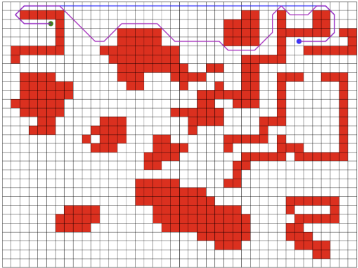
\includegraphics[width=0.6\textwidth]{Ataidhawijd.png} % 
\caption{Greedy Search (pink) Behaving Suboptimally Relative to A* (blue). Credit: Ben's 16.410 PSET. }
\end{center}
\label{workflow}
\end{figure}}
We thus settled on A* as our path planning algorithm were we to choose a graph-based algorithm. \\



\textbf{Final Decision: RRT/RRT* vs A*}. We thus had narrowed down our choice to RRT or RRT* if we wanted a sample-based algorithm and A* if we wanted a graph-based algorithm. In the case of a racecar, intuitively it seems as though random paths aren't great. Especially in a competitive environment where time determines the winners, a non-optimal (or far from optimal at least) path is not great. Figure 3 shows two images of RRT running in a randomly generate envirornment. 


\textbf{\begin{figure}[H]
\begin{center}
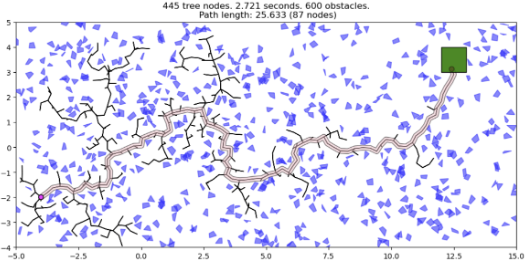
\includegraphics[height=0.28\textwidth]{RRT1.png} % 
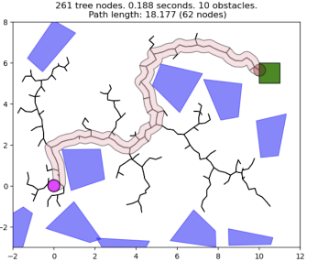
\includegraphics[height=0.28\textwidth]{RRT2.png} % 
\caption{RRT (with Goal Biasing) Visualization in Two Random Environments. Credit: Ben's 16.410 PSET. }
\end{center}
\label{workflow}
\end{figure}}



As shown, RRT can produce some strange paths. While RRT* is \textit{asymptotically optimal}, in that paths approach optimality as the number of nodes in the tree approaches infinity, it also sacrifices some of the runtime of RRT, and in practice we would not allow RRT* to run long enough to reach an optimal solution. This limits the benefits of RRT* over RRT. Given that the requirement for runtime of our path planning algorithm was 120 seconds, we decided that we would implement a A* with the intent of preferring a good path over planning speed. A* is additionally desirable because computing an admissable heuristic (euclidean distance) is significantly easier than some of the necessary computations for RRT (i.e. collision checking). Additionally, while the asymptotic runtime of A* is $O(b^m)$, in practice, and with a good heuristic, A* is often not \textit{very} slow and can compute short paths very quickly. However, the choice of algorithm depends largely on context! If our main goal was to quickly plan a path - or if planning time was included in the competition (i.e. time to goal includes planning time) then it may have been a better choice to use a sampling-based algorithm.  \\





% Explain path planning algorithms, and the strengths and weaknesses of sample-based versus search-based methods. Which algorithm should work better for the purposes of planning trajectories for your car? What different cost functions would you use? How would you ensure the car would not choose paths close to the wall?
%Specifically, please discuss the following properties of planning algorithms, along with any others you considered: asymptotic optimality, single- vs multi-query, incorporating dynamics, complexity, and necessity of search after construction. Note that some of these are only applicable to search-based planners and some are only applicable to sampling-based planners.

\subsubsection{A* Implementation}
We implemented a standard A* algorithm to plan paths. We used python \textit{heapq} to create a min-heap as our queue structure. We used the implicit grid structure provided by the given map, which has about 2 million nodes, and did not downsample. Although we expected to have to condense the grid, it turned out that A* ran quick enough without condensing the grid space. We only consider free neighbors, and we maintain a visited list to cut down on runtime. We used euclidean distance as an admissable heuristic. In practice this worked well. If we wanted a more accurate heuristic, we could use dublin curves, which take into account the dynamics of a wheeled vehicle. We defined the neighbors of a node in grid space as it's 8 surrounding nodes in grid space; thus the car can go up, down, left, right, or diagonally at 45 degrees, from a given point in space. It could be better to consider transitions at different angles, but this could also be accomplished by applying a splining operation after creating the path. \\

\textbf{Map Dilation}: In order to account for real-world dynamics, errors in localization, and the 'cutting-corner' tendencies of pure-pursuit, we planned our paths on a dilated version of the map. That is, we enlarged obstacles past their actual dimensions; thus, when a path is planned, the path stays farther away from the actual obstacles. We dilated by converting to a binary image and using a 15 x 15 kernel of 1's during dilation. Figure 4 shows the effect of dilation.  

\textbf{\begin{figure}[H]
\begin{center}
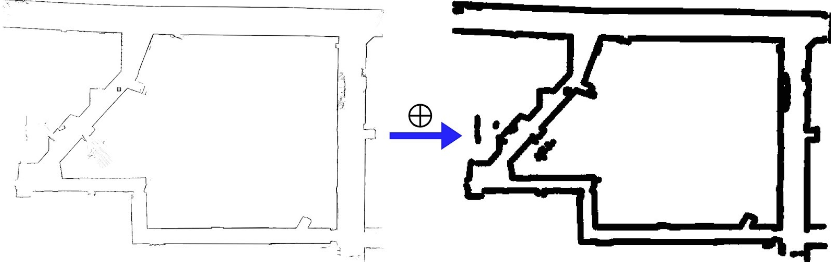
\includegraphics[height=0.28\textwidth]{dilation.png} % 
\caption{Map Dilation Example. Credit: MIT RSS Github. }
\end{center}
\label{workflow}
\end{figure}}
In practice, map dilation worked very well at ensuring the car did not get too close to an obstacle. 
\newpage
\subsubsection{A* Performance}
A* worked well at planning paths! In Figure 5 some example paths are shown. In practice, a short path took 0-1 seconds to create, and the longest possible path (corner to corner) took $\approx$ 10 seconds to create. 

\textbf{\begin{figure}[H]
\begin{center}
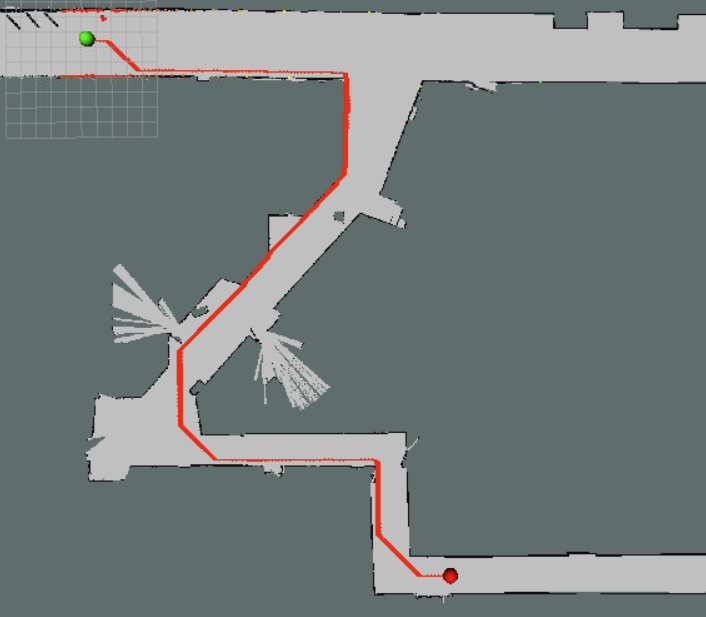
\includegraphics[height=0.23\textwidth]{Screenshot 2023-04-18 224740.png} % 
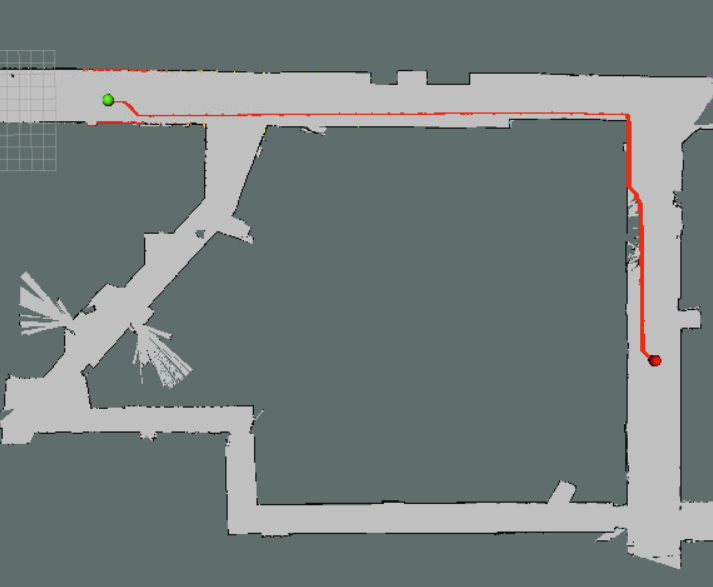
\includegraphics[height=0.23\textwidth]{Screenshot 2023-04-18 224834.png} % 
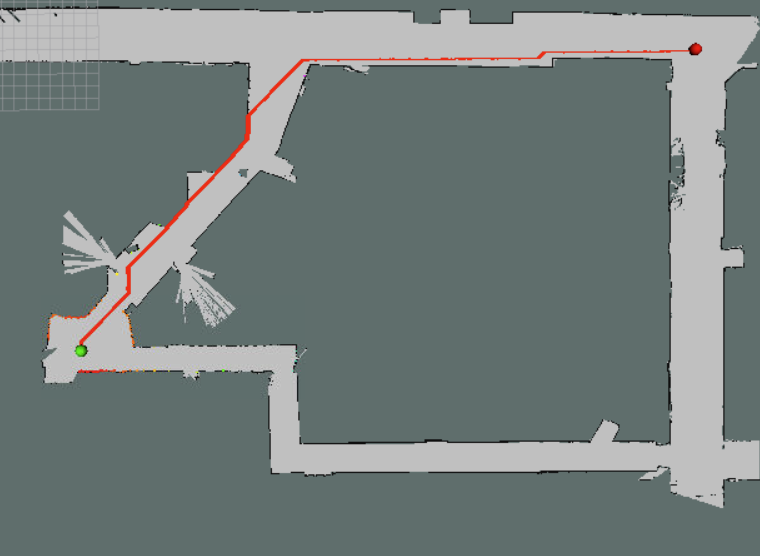
\includegraphics[height=0.23\textwidth]{Screenshot 2023-04-18 224913.png} % 
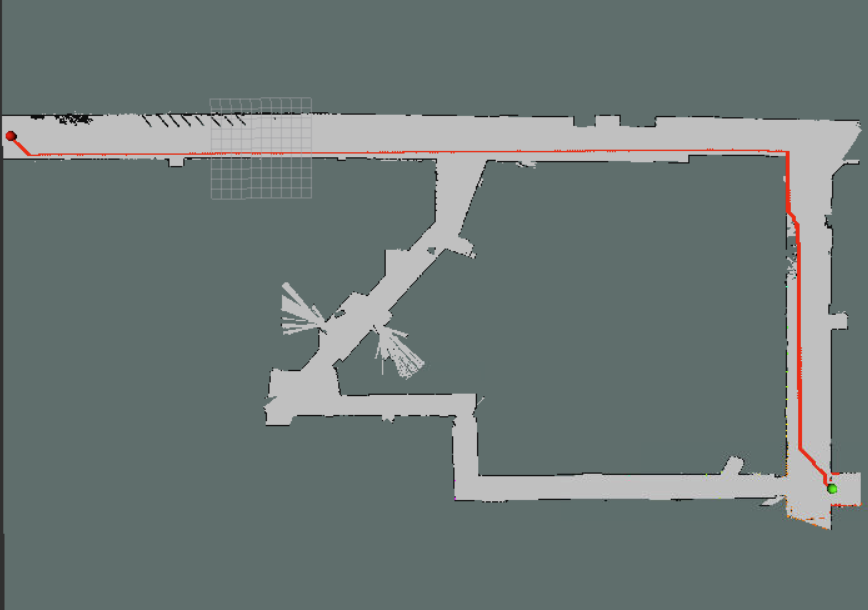
\includegraphics[height=0.23\textwidth]{Screenshot 2023-04-18 225026.png} % 
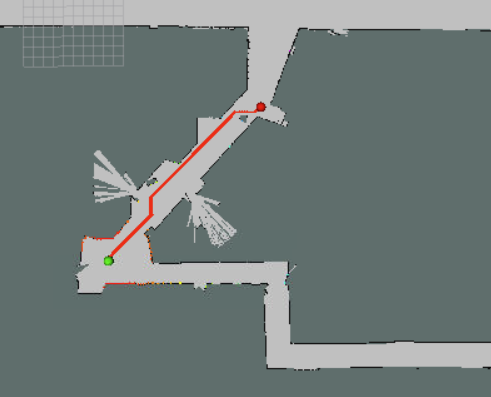
\includegraphics[height=0.23\textwidth]{Screenshot 2023-04-18 225459.png} % 
\caption{Examples of A* Path Planning. The Green Dot denotes the start point. The Red Dot denotes the endpoint. }
\end{center}
\label{workflow}
\end{figure}}


\textbf{Comments on Optimality}: As shown in Figure 5, the paths created are not perfectly optimal. This is expected. As explained in "Sample-Based Path Planning Algorithms", A* is only guaranteed optimal with a visted list if we use a \textit{consistent} heuristic. We are using euclidean distance, which is an \textit{admissable} but not consistent heuristic. However, because our graph has so many nodes with very close neighbors, the paths wind up being very good, as there exist multiple good paths to the goal! Thus, using a visited list with an admissable heuristic combines quick execution time with very good (but not optimal) paths. In other words, we compromise on perfect optimality a small amount to help runtime significantly.











\subsection{Pure Pursuit (Author: Steven Liu)}

Given a (piecewise linear) trajectory, we now need to determine the drive commands necessary to follow it. While more advanced tracking algorithms exist, one which is simple and very flexible is pure pursuit, which we found to provide sufficient performance. \\

At a high level, pure pursuit is very straightforward. The car determines a point on the track ahead of it to be its target point, and attempts to drive directly towards it. Once the point is found, the driving is accomplished simply by turning the front wheels to point directly at the target point and driving forwards at a constant, designated speed. This continues until the car is within some defined distance of the final point in the trajectory. \\

\textbf{\begin{figure}[H]
\begin{center}
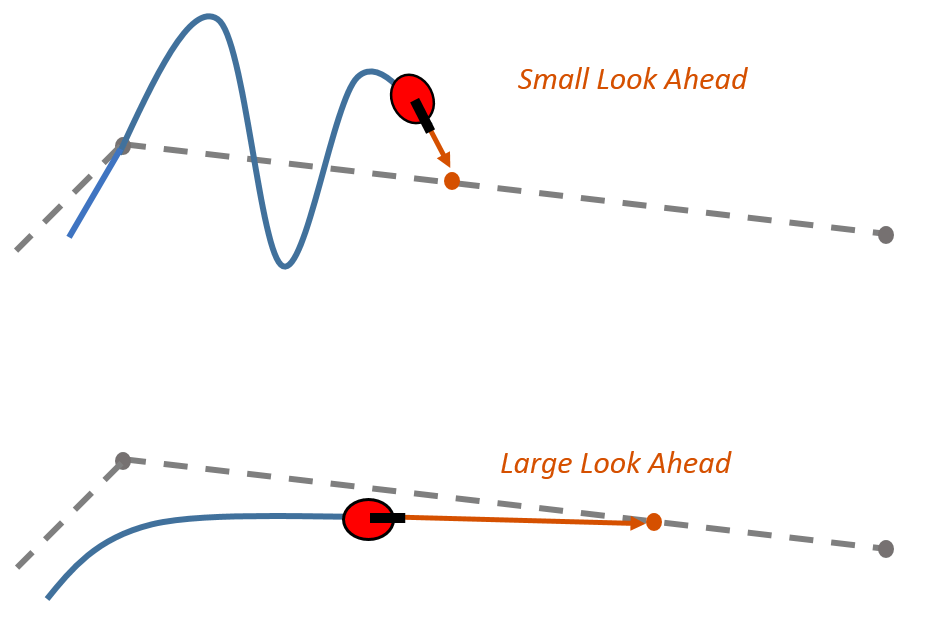
\includegraphics[height=0.4\textwidth]{pure_pursuit_lookahead2.png} % 
\caption{Pure pursuit lookahead. Credit: Mathworks. }
\end{center}
\label{lookahead}
\end{figure}}

Finding the target point is somewhat more involved. The first step is to determine where along the trajectory the car is. Because in general the car will not be exactly on the trajectory, it is necessary to calculate where the closest point on the trajectory to the car is. The piecewise linear nature of the trajectory can be taken advantage of here: each linear segment has exactly one closest point to the car, which is straightforward to determine with some geometry. The closest point on the entire trajectory naturally must be the closest point on one of the segments; thus, we may iterate through the segments for the closest point. \\

The first case, given a closest point, is that the point is farther from the car than the lookahead distance. When this happens, that means the car is substantially off-course. To remedy this, drive commands are given to drive towards the closest point so as to get the car back on track as quickly as possible. \\

The other case is that the closest point is within the lookahead distance. In this case, we can then check each segment including and after the one containing the closest point in turn to determine whether it intersects the lookahead circle. The search stops after the first such intersection is found, after which the intersection point is returned as the target point. If no intersection is found, then that means the rest of the trajectory is entirely contained within the lookahead circle, and the car may simply drive directly to the end.

\subsection{Integration to Racecar} 

Surprisingly, integrating Pure Pursuit, Path Planning, and Localization onto the racecar was very smooth. We had to dial-in the dilation a bit, which took some iteration. However, other than this and some parameter adjustments to pure pursuit, everything worked almost immediately when integrated. 

\subsection{Summary}
Overall, we thought considerably about how to tackle this lab. e ultimately decided on A* as our path planning algorithm. By communicating extensively on inputs and outputs, we ensured that racecar implementation went smoothly!



\newpage
\section{Experimental Evaluation (Author: Dinuri Rupasinghe)}
% WHOEVER WRITES SECTION: please reference the necessary checkpoints for this section on the git lab description

\subsection{Overview}
In order to evaluate the performance of our racecar in path planning and pure pursuit, we used two main metrics. The first metric was the gradescope autograder, which was given by the RSS faculty to evaluate our algorithms via simulation. The second metric was the error calculations garnered by the real life performance of our racecar. Some quantitative performance metrics that were used in simulation were assuring that the planning time was within 120 seconds and pursuit time was within 500 seconds. Qualitatively, we made sure that our racecar avoided occluded space on the map and in general, avoided collisions and obstacles. 

\subsection{Path Planning Tests}
In order to test our A* path planning algorithm, we used the rviz controls to plot a goal point to navigate to, as well as plot our starting point with respect to where our racecar was positioned in real life. The following points were selected and the trajectories that were developed from our path planning algorithm are shown.\\

In Figure 7: Path Planning Test 1, a path was formed without colliding into any obstacles. The racecar chose a path that had the smallest distance to the goal point. Next, in Figure 8: Path Planning Test 2, the racecar was to trek through a more harsh environment. This included more obstacles like columns, jagged walls, and sharp turns. The racecar was still able to successfully form a short path through the harsh environment, without taking the simpler but longer path from the other side of the Stata basement. Lastly, in Figure 9: Path Planning Test 3, the racecar was to trek through a similar harsh environment, except this time involved many more harsh turns. One is able to see that a path was able to be formed without running into any obstacles. At many appropriate points the car took practical measures to follow the most efficient side of the wall, and also cross to switch the sides of the wall in which it was following. \\
\\
% WHOEVER WRITES THIS SECTION GET PLOTS FROM (1) running path planning yourself and showing it plan a path in diff scenario, (2) ask ben to send you some plots, (3) pull plots from the presentation. 
\textbf{\begin{figure}[H]
\begin{center}
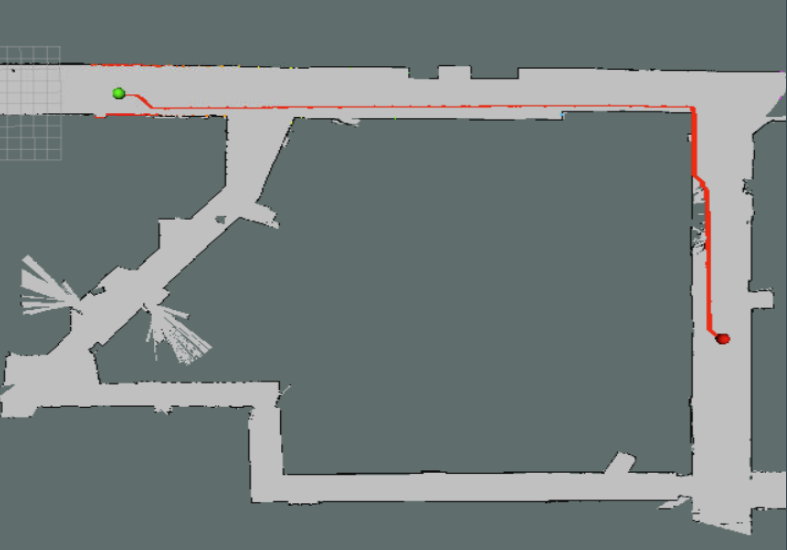
\includegraphics[width=0.4\textwidth]{pp2.png} % 
\caption{Path Planning Test 1: Simple Turn}
\end{center}
\label{workflow}
\end{figure}}
\textbf{\begin{figure}[H]
\begin{center}
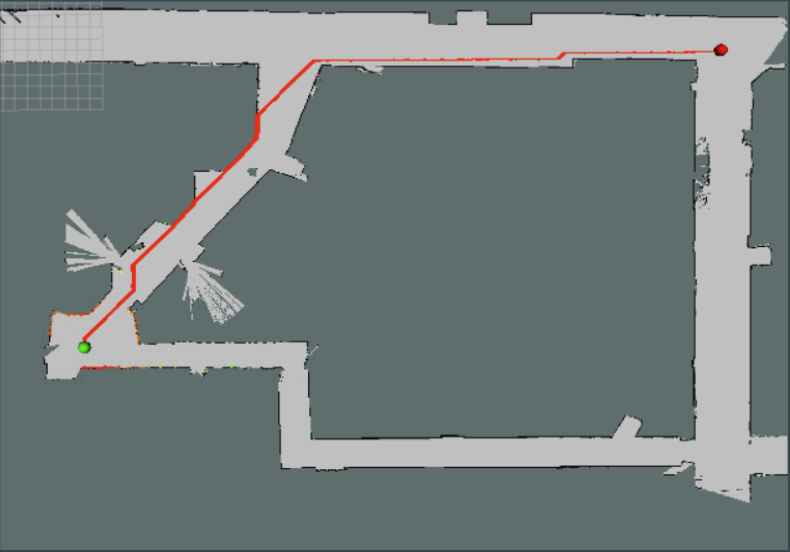
\includegraphics[width=0.4\textwidth]{pp3.png} % 
\caption{Path Planning Test 2: Some Obstacles}
\end{center}
\label{workflow}
\end{figure}}
\textbf{\begin{figure}[H]
\begin{center}
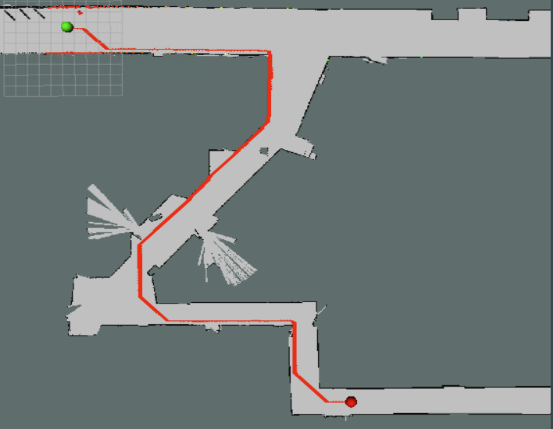
\includegraphics[width=0.4\textwidth]{pp1.png} % 
\caption{Path Planning Test 3: Complex Corners and Obstacles}
\end{center}
\label{workflow}
\end{figure}}


\subsection{Pure Pursuit Tests}
%WHOEVER WRITESTHIS SECTION GET PLOTS FROM (1) running pure pursuit in sim yourself, (2) asking steven for some good plots
The testing of our pure pursuit algorithm was tested by testing through the gradescope autograder and in real life through our video demonstrations, as one will see below. When assessing the performance of pure pursuit, we made sure to pay careful attention to how far off the racecar was from the planned path at all times. Additionally, an important metric to take into account in real life is the ability of our racecar to move smoothly. For example, we did not want our racecar to have oscillatory behavior, run into walls, steer for turns too late. We accounted for these qualitative metrics by increasing look-ahead distance and also dilating our map. Please see information for Figure 11, Figure 14, and Figure 15 for quantitative metrics on our pure pursuit testing.

\subsection{Gradescope Autograder}
In the gradescope autograder, we were able to test our algorithms in simulation before integrating it to the racecar. This procedure was particularly helpful in testing the algorithm first in order to assure our racecar would not run into any walls in the maps given. In all of our gradescope tests, a particle filter code was necessary, and we would like to note that we utilized our own particle filter code, rather than the TA solution.\\

It is important to note how the gradescope autograder obtained scores from our implementation. There were several metrics used. First, planning time and pursuit time were to be within \emph{plan time thresh} (120 seconds) and \emph{pursuit time thresh} (500 seconds). Secondly,the cumulative distance of the path traversed was to be within \emph{delta path max*path length} (2 times the path length). Lastly, the amount of time spent driving within delta pursuit (set at 1 meter) heavily factored into the score. \\
\\
\textbf{\begin{figure}[H]
\begin{center}
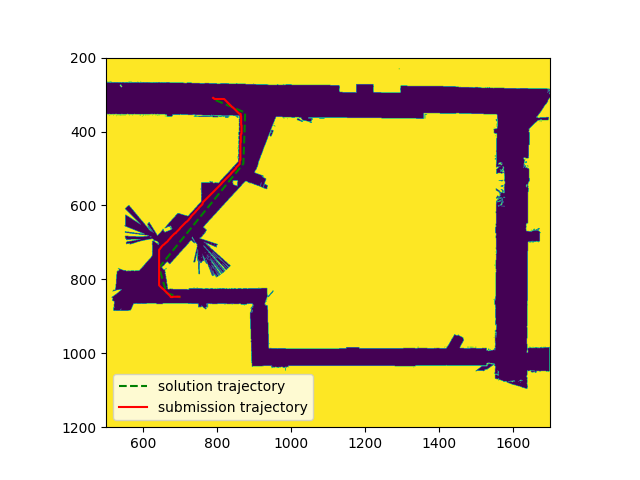
\includegraphics[width=0.6\textwidth]{path planning.png} % 
\caption{Path Planning Test on Gradescope Autograder. Score: 95.2/100}
\end{center}
\label{workflow}
\end{figure}}
The gradescope autograder tested our path planning algorithm alone at first, meaning that there was no pure pursuit of a path and only trajectory planning was tested. We received a score of 95.2 out of 100 on this solution. (See Figure 10) It is quite close to the TA solution, as there is almost complete overlap with the solution trajectory and the submission trajectory. \\
\textbf{\begin{figure}[H]
\begin{center}
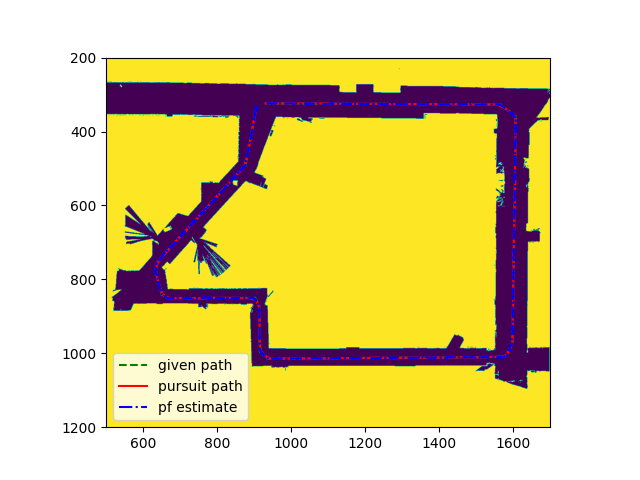
\includegraphics[width=0.6\textwidth]{pure pursuit test.png} % 
\caption{Pure Pursuit Test on Gradescope Autograder. Score: 95.1/100}
\end{center}
\label{workflow}
\end{figure}}
The gradescope autograder also tested pure pursuit alone. This meant that a trajectory was planned out for our simulation, and the autograder tested how well we could pursue the given path. (See Figure 11) One can see that the given path has complete overlap with the pursuit path, as we cannot see the green dotted line. A quantitative observation yields that our pure pursuit algorithm received a score of 95.1 out of 100.\\

Lastly, the gradescope autograder tested both our path planning algorithm and pure pursuit algorithm together. Here, our work received a score of 97 out of 100. Our pursuit path overlaps with the TA solution for a given path almost completely.

\textbf{\begin{figure}[H]
\begin{center}
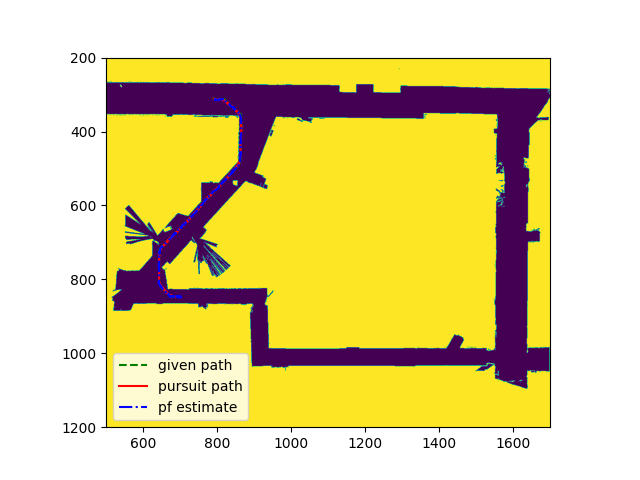
\includegraphics[width=0.6\textwidth]{both test.png} % 
\caption{Path Planning and Pure Pursuit Tested Together on Gradescope Autograder. Score: 97/100}
\end{center}
\label{workflow}
\end{figure}}


\subsection{Video Demonstrations}
Here is the \href{https://drive.google.com/file/d/1gFyXzFMGskptzbs8HqVI4FKhudgxbtVI/view?usp=}{\underline{link to our video demonstrations of our car}.} In our video demonstrations, our goal was to prove that the car could plan a path and pursue the path in real life. Thus, our videos show our racecar moving from start to finish in real life with the path planned in simulation and error plots of the distance the car is from the preplanned path.\\
\\
\textbf{\begin{figure}[H]
\begin{center}
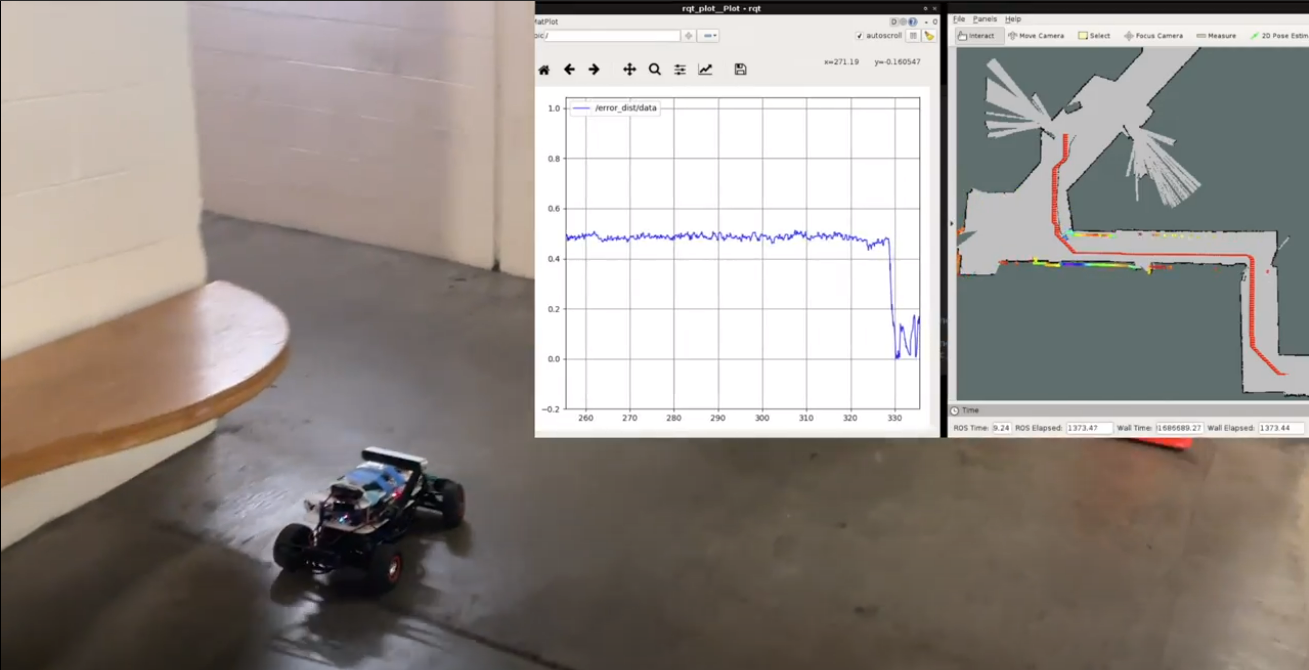
\includegraphics[width=0.7\textwidth]{demowithcar.png} 
\caption{Image of our video demonstration, depicting racecar in real life, the path planned, and an error plot.}
\end{center}
\label{workflow}
\end{figure}}

In our real life implementation of our algorithms on our car, we were able to test two possible start and end goals. The red path signifies the path planned by our path planning algorithm. The dotted black line signifies the path traversed by our car in following our pure pursuit algorithm. We obtained an RQT plot of the error obtained when traversing the path planned. The error describes how far off the racecar veers off the planned path. In Demo 1, (Figure 14) we were ale to test a somewhat challenging path with a few turns. We were able to correctly follow our planned path, with an error on average within 0.3 meters. One may also notice that there is a large error when Demo 1 first commences. This is due to the fact that we placed the racecar a bit away from the starting point we chose in rviz, and the error is large but quickly decreases as the racecar navigates to the proper starting position. 
\\
\\
In Demo 2, (Figure 15) we were able to test a more complex path with obstacles, including a large column which was somewhat difficult to traverse. We were able to correctly follow our planned path, with an error on average within 0.3 meters. In both demos, one can see that a practical, relatively short path was generated when the start and end points were manually chosen by our team on the map. 

\textbf{\begin{figure}[H]
\begin{center}
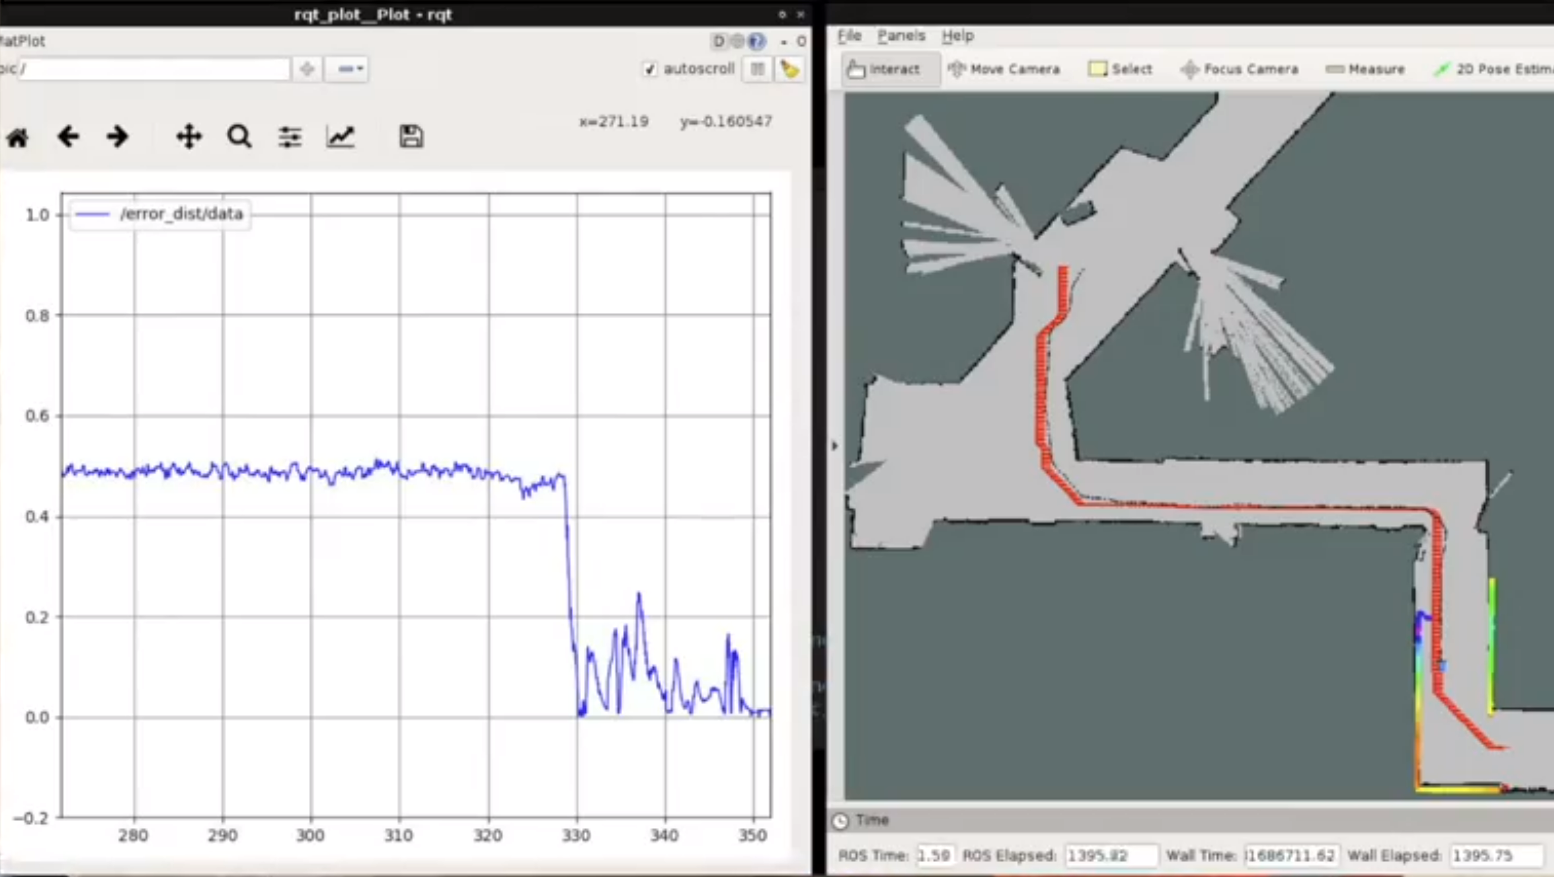
\includegraphics[width=0.7\textwidth]{demo1.png} 
\caption{Demo 1}
\end{center}
\label{workflow}
\end{figure}}
\textbf{\begin{figure}[H]
\begin{center}
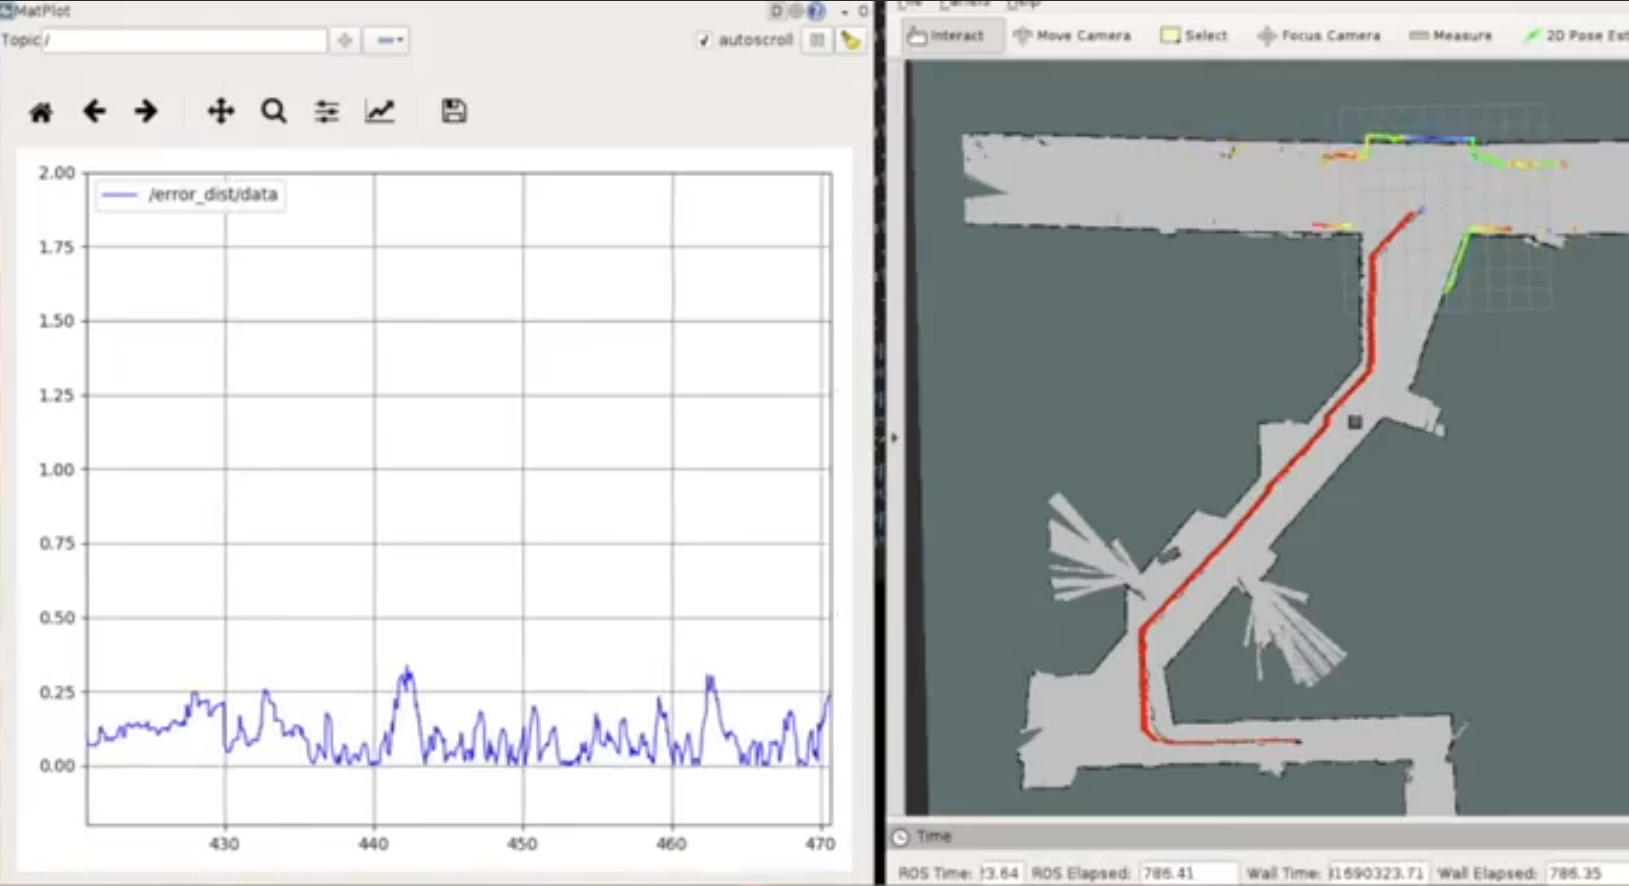
\includegraphics[width=0.7\textwidth]{demo2.png} 
\caption{Demo 2}
\end{center}
\label{workflow}
\end{figure}}

\subsection{Summary}
Overall, we were able to evaluate the performance of our racecar through various metrics, including the gradescope autograder and error plots from our real life testing. Our racecar was able to successfully create an efficient path and follow the path within and error of 0.3 meters at all times. Our car is robust to most difficult turns and obstacles.


\section{Potential Improvements (Author: Jose Soto)}

As we approach the final challenge, which we predict will have a variety of unique obstacles, we anticipate that we will have to make various improvements to improve the fidelity and robustness of our path finding software. \\

Overall, one of the improvements that our group will consider implementing in our algorithm is improving our current A* heuristic. We are currently using shortest euclidean distance, and this works well for our current model. To improve efficiency and speed we are looking into different heuristics, including dubins curves. This heuristic more accurately accounts for vehicle dynamics, which we anticipate improving the speed and performance of our car if implemented. \\

We use a primitive dilation technique, simply dilating it to "squares" around the map we were given. We anticipate that a different shape for dilation, like discs, will be much more condusive to corners and improve the turning efficiency of our path planning algorithm.\\

Our implementation on the hardware also has the downside oscillatory behavior. This is a problem we anticipate could have various different effects. One of them is our current path planning algorithm, and the sharp turns that are made as a result of not "smoothing" out the edges of the path. These sharp turns lead to our car over correcting to the path, leading to oscillatory behavior. We believe that once we smooth out the path and tweak some parameters of our pure pursuit algorithm, we can see smooth turning: vastly improving our cat's speed. \\

In order to smooth out the path, we will take the path given to us by the A* algorithm and apply a splining procedure to it, replacing the sharp corners with much more gradual splines that more accurately represents how a vehicle moves in physical space. This will allow us to take corners at higher speeds, and reduces the oscillatory effects seen in this lab. \\
\section{Conclusion (Author: Sophia Wang)}

Overall, our team can confidently say that we developed and implemented path planning for our vehicle. We were successfully able to implement both components: planning trajectories in a known occupancy grid map to a goal pose using a graph-based motion planning method and implementing pure pursuit on the car to follow the computed trajectory. Path planning meets several quantitative and qualitative performance metrics, including computing and executing planning and pursuit goal trajectories within timeout thresholds and error and distance margins, avoiding occluded space on the map, and avoiding collisions and obstacles. Integration with previously developed localization and safety control modules also proved successful and robust in integration onto hardware. \\

Looking ahead, our team has a few improvements to be made in preparation for our final deliverable at the end of the course which includes: improving our dilation technique, reducing oscillations in the robot's pure pursuit of trajectories, and conducting further post-processing on generated paths to remove sharp turns. In the upcoming weeks, we will test the robot's performance with the aforementioned improvements on the given competition track.

\section{Lessons Learned}
%Presents individually authored self-reflections on technical, communication, and collaboration lessons you have learned in the course of this lab.

\subsection{Benjamin Rich}
This was a pretty fun lab. It was interesting how well each module came together. Working on path planning, then using it to debug pure pursuit was smart, and somehow everything came together quickly on the actual car. I think the biggest take away from this lab is that driving a strict schedule is important for finishing on time. By avoiding having to push back our briefing, we gained more time to start thinking about the final challenge. I think this will very much help us avoid a stressful end to the semester!

\subsection{Dinuri Rupasinghe}
The path planning lab was interesting. I had learned about different path planning algorithms in some classes before, so it was definitely interesting to implement an algorithm for our car. I found the integration of our algorithms onto our car particularly interesting because implementing our work in simulation proved to be quite different than in real life. Overall, I am thankful that we decided to finish the software components of the lab and implement onto our actual racecar early, as this helped us finish the lab efficiently.

\subsection{Sophia Wang}
This lab was rewarding, especially during our final phase of integrating onto hardware. Seeing the planned trajectory mapped in rviz and simulation and then seeing the automation happen (the car steering itself towards the goal pose) was a fun transition. Additionally, it was gratifying to successfully integrate multiple modules developed throughout the semester, such as last lab's localization and our first group lab's safety controller. We got good feedback from our briefing regarding improvements prior to the final challenge, and we look forward to integrating these!

\subsection{Steven Liu}

While I would have liked to try out some more advanced planning and following algorithms, what we did accomplish was still well above my expectations coming into the lab. It was especially satisfying testing our localization code on a real application it wasn't initially designed for, and while it wasn't perfect, the fact that we could just use it as-is is to me an indication that we did the last lab very well. We were perhaps lucky that integration on the car was almost seamless, since we may have been tight on time if we had to make significant changes. That said, since we got this lab done so fast, we've gotten a good head start on the final challenge and working on the car for that.

\subsection{Jose Soto}
I found this lab pretty satisfying. It was great to immediately see the results of the previous lab, localization, coming into play and being used to localize and locate the car with respect to the path. Also, the ability to visualize the car's path and follow it in real time (and edit a video showing that) is super fun to watch. Since we finished the lab early, we had a lot of time to reflect and work on the next lab promptly, which I anticipate is going to really improve the quality of our final product- which I am extremely excited to see culminate all of the knowledge we've gained from the labs.
\newpage 
\section{Appendix}
\subsection{Path Planning Code}

{\footnotesize
\begin{verbatim}
    #!/usr/bin/env python

import rospy
import numpy as np
from geometry_msgs.msg import PoseStamped, PoseArray, Point, PoseWithCovarianceStamped
from nav_msgs.msg import Odometry, OccupancyGrid
import rospkg
from scipy import ndimage
import time, os
#import dubins
import tf
from utils import LineTrajectory
from graph_class import Graph
import heapq
#import cv2 
#from skimage import morphology

#### NOTE: later on we should try dublin curves, nice package in the git for this...
# roslaunch racecar_simulator simulate.launch
# roslaunch lab6 plan_trajectory.launch
# sudo apt-get install python-scipy


# TODO: figure out dilation in gradescope? idk
class PathPlan(object):
    """ Listens for goal pose published by RViz and uses it to plan a path from
    current car pose.
    """
    def __init__(self):

        self.start_pos = None
        self.goal_pos_irl = None
        self.goal_pos_map = None
        self.graph = None
        self.map = None
        self.map_coords = None
        self.height = None
        self.width = None
        self.start_time = None

        self.odom_topic = rospy.get_param("~odom_topic")
        #self.odom_topic = '/odom' # FOR TESTING ONLY - on real car, change to listen to localization shit... is this right?
        self.map_sub = rospy.Subscriber("/map", OccupancyGrid, self.map_cb)
        self.trajectory = LineTrajectory("/planned_trajectory")
        self.goal_sub = rospy.Subscriber("/move_base_simple/goal", PoseStamped, self.goal_cb, queue_size=10)
        self.traj_pub = rospy.Publisher("/trajectory/current", PoseArray, queue_size=10)
        self.odom_sub = rospy.Subscriber(self.odom_topic, Odometry, self.odom_cb) #TODO: MAKE THIS FUNCTIONAL
        self.intial_pose_sub = rospy.Subscriber('/initialpose',PoseWithCovarianceStamped, self.initial_pose_cb, queue_size=10)

        self.rot_matrix = None
        self.rot_alt = None
        self.rot_back = None
        self.rot_back_alt = None
        self.heuristic = None
        self.map_res = None

    def pixelToMapCoords(self,u,v):
        u *= self.map_res; v *= self.map_res
        x,y,_ = np.matmul(np.array([[u,v,0]]),self.rot_alt)[0]
        return x+self.rot_matrix[0][3], y+self.rot_matrix[1][3]
    
    def mapToPixelCoords(self,x,y):
        u,v,_  = np.matmul(np.array([[x,y,0]]),self.rot_back_alt)[0]
        x = (u+self.rot_back[0][3])/self.map_res; y = (v+self.rot_back[1][3])/self.map_res
        return int(np.rint([x])[0]), int(np.rint([y])[0])

    def eucDist(self,coord1,coord2): 
        return np.sqrt((coord1[0]-coord2[0])**2+(coord1[1]-coord2[1])**2)

    def map_cb(self, msg):
        map = np.reshape(np.array(list(msg.data)),(msg.info.height, msg.info.width)).astype('uint8') # convert from row-major order
        self.map_res = msg.info.resolution; self.height = np.shape(map)[0]; self.width = np.shape(map)[1]
        map_copy = map[:]
        # DEFINE ROTATION STUFF
        rot_matrix = tf.transformations.quaternion_matrix([0, 0, msg.info.origin.orientation.z, msg.info.origin.orientation.w])
        rot_matrix[0][3] = msg.info.origin.position.x; rot_matrix[1][3] = msg.info.origin.position.y; rot_matrix[2][3] = msg.info.origin.position.z
        rot_alt = [rot_matrix[0][0:3],rot_matrix[1][0:3],rot_matrix[2][0:3]]
        self.rot_matrix = rot_matrix; self.rot_alt = rot_alt; self.rot_back = np.linalg.inv(self.rot_matrix); self.rot_back_alt = np.linalg.inv(self.rot_alt)

        # dilate
        map[map > 0] = 1; map[map < 0] = 1
        map_copy = map[:]
        kernel = np.ones((10, 10), np.uint8) # 28,28
        map = ndimage.binary_dilation(map,structure=kernel)
        x = 40
        map[767-x:767+x,423-25:423+25]=map_copy[767-x:767+x,423-25:423+25]
        self.map = map
        print('### MAP INITIATED ###')

    def initial_pose_cb(self,data):
        u,v = self.mapToPixelCoords(data.pose.pose.position.x,data.pose.pose.position.y)
        if  (u,v) != self.start_pos:
            print('### new start(init)' + str((u,v))+' ### ')
            self.start_pos = (u,v)

    def odom_cb(self, data): # NOTE: not sure what this callback should be doing?
        #if self.rot_back_alt == None or self.rot_back == None or self.map_res == None: return
        u,v = self.mapToPixelCoords(data.pose.pose.position.x,data.pose.pose.position.y)
        self.start_pos = (u,v)


    def goal_cb(self, data):
        theta = 2*np.arctan2(data.pose.orientation.z,data.pose.orientation.w)
        self.goal_pos_irl = (data.pose.position.x,data.pose.position.y,theta)
        self.trajectory = LineTrajectory("/planned_trajectory")
        u,v = self.mapToPixelCoords(self.goal_pos_irl[0],self.goal_pos_irl[1])
        self.goal_pos_map = (u,v) 
        print('### set new goal:'+str(self.goal_pos_map)+' ###')
        self.plan_path((self.start_pos[0],self.start_pos[1]),self.goal_pos_map,self.map)


    def AStarWithExpandedListPartialPaths(self,map,S,G):
            
            def computeH(u,v): 
                return self.eucDist((u,v),(self.goal_pos_map[0],self.goal_pos_map[1]))
            
            def getChildren(i,j):
                return [(i+1,j),(i-1,j),(i,j+1),(i,j-1),(i+1,j+1),(i-1,j-1),(i+1,j-1),(i-1,j+1)]

            expanded = set()
            Q = [(computeH(S[0],S[1]),(0,[S]))] # (cost_to_come+cost_incurred,(cost_incurred, head))
            heapq.heapify(Q)
            while Q:
                _, N = heapq.heappop(Q)
                partial_path = N[1]; costIncurred = N[0]
                head = partial_path[-1]
                if head == G:
                    return costIncurred, partial_path
                elif head in expanded:
                    continue
                else:
                    expanded.add(head) # NOTE: check!
                    children = getChildren(head[0],head[1])
                    for child in children:
                        if child not in expanded:
                            try:
                                if map[child[1]][child[0]] == 0:
                                    new_partial = partial_path[:]
                                    new_partial.append(child)
                                    costToChild = self.eucDist(head,child) + costIncurred
                                    heapq.heappush(Q,(costToChild+computeH(child[0],child[1]),(costToChild,new_partial)))
                                else:
                                    expanded.add(child)
                            except: # out of bounds
                                continue             
            return None, None

    def plan_path(self, start_point, end_point, map):
        print('planning path.......')
        self.start_time = rospy.get_time()
        _, partialPath = self.AStarWithExpandedListPartialPaths(map,start_point,end_point)
        print('finished planning path, time = '+str(rospy.get_time()-self.start_time))
        
        if partialPath is not None:
            for node in partialPath:
                point = Point()
                x1,y1 = np.round(self.pixelToMapCoords(node[0],node[1]),decimals =2)
                point.x = x1; point.y = y1; point.z = 0.0
                self.trajectory.addPoint(point)
                # publish traj and visualize
            self.traj_pub.publish(self.trajectory.toPoseArray())
            self.trajectory.publish_viz()
        else:
            print('ERR: failed to find path')


if __name__=="__main__":
    rospy.init_node("path_planning")
    pf = PathPlan()
    rospy.spin()

\end{verbatim}
}
\subsection{Pure Pursuit Code}
{\footnotesize
\begin{verbatim}
#!/usr/bin/env python

import rospy
import numpy as np
import time
import utils
import tf

from std_msgs.msg import Float32
from geometry_msgs.msg import PoseArray, PoseStamped
from visualization_msgs.msg import Marker
from ackermann_msgs.msg import AckermannDriveStamped
from nav_msgs.msg import Odometry

eucl_dist = lambda a,b: ((a[0]-b[0])**2+(a[1]-b[1])**2)**0.5

class PurePursuit(object):
    """ Implements Pure Pursuit trajectory tracking with a fixed lookahead and speed.
    """
    def __init__(self):
        self.odom_topic       = rospy.get_param("~odom_topic")
        self.lookahead        = 1 # FILL IN #
        self.speed            = 1 # FILL IN #
        self.wheelbase_length = 1 # FILL IN #
        self.trajectory  = utils.LineTrajectory("/followed_trajectory")
        self.traj_sub = rospy.Subscriber("/trajectory/current", PoseArray, self.trajectory_callback, queue_size=1)
        self.drive_pub = rospy.Publisher("/drive", AckermannDriveStamped, queue_size=1) # /vesc/ackermann_cmd_mux/input/navigation
        self.odom_sub = rospy.Subscriber(self.odom_topic, Odometry, self.odometry_callback, queue_size=1)
        self.error_pub = rospy.Publisher("/error_dist",Float32,queue_size=10)
    def trajectory_callback(self, msg):
        ''' Clears the currently followed trajectory, and loads the new one from the message
        '''
        print "Receiving new trajectory:", len(msg.poses), "points"
        self.trajectory.clear()
        self.trajectory.fromPoseArray(msg)
        self.trajectory.publish_viz(duration=0.0)

    def odometry_callback(self, msg):
        '''
        Given a pose estimate from the localization package,
        figure out where to drive to, and make the appropriate drive command
        '''
        if self.trajectory.empty(): return
        
        pose = (msg.pose.pose.position.x,msg.pose.pose.position.y)
        
        # find target point
        nearest_point_index = None
        nearest_point = None
        nearest_dist = float('inf')
        for i in range(len(self.trajectory.points)-1):
            # Always check endpoints of current segment
            crit_points = [self.trajectory.points[i],self.trajectory.points[i+1]]
            
            # Parameterize the line and determine if an interior point is a critical point
            dx,dy = self.trajectory.points[i+1][0]-self.trajectory.points[i][0],\
                    self.trajectory.points[i+1][1]-self.trajectory.points[i][1]
            x0,y0 = self.trajectory.points[i][0]-pose[0],self.trajectory.points[i][1]-pose[1]
            t = -(x0*dx+y0*dy)/(dx**2+dy**2)
            if t > 0 and t < 1:
                crit_points.append((t*self.trajectory.points[i+1][0]+(1-t)*self.trajectory.points[i][0],
                                    t*self.trajectory.points[i+1][1]+(1-t)*self.trajectory.points[i][1]))
            
            # Test each critical point
            for j in range(len(crit_points)):
                dist = eucl_dist(crit_points[j],pose)
                if dist < nearest_dist:
                    nearest_dist = dist
                    nearest_point = crit_points[j]
                    if j == 0: nearest_point_index = i
                    elif j == 1: nearest_point_index = i+1
                    elif j == 2: nearest_point_index = i+t
        
        # If we're too far from the track, beeline to the nearest point
        self.error_pub.publish(nearest_dist)
        if nearest_dist >= self.lookahead:
            target_point = nearest_point
        else:
            # Otherwise, find the first point after the nearest point outside the circle
            for i in range(int(nearest_point_index)+1,len(self.trajectory.points)):
                if eucl_dist(self.trajectory.points[i],pose) > self.lookahead:
                    # Find intersection of the line with the target circle closer to the next point
                    dx,dy = self.trajectory.points[i][0]-self.trajectory.points[i-1][0],\
                            self.trajectory.points[i][1]-self.trajectory.points[i-1][1]
                    x0,y0 = self.trajectory.points[i-1][0]-pose[0],self.trajectory.points[i-1][1]-pose[1]
                    a,b,c = dx**2+dy**2,2*(x0*dx+y0*dy),x0**2+y0**2-self.lookahead**2
                    t = (-b+(b**2-4*a*c)**0.5)/(2*a)
                    assert t >= 0 and t <= 1
                    target_point = (t*self.trajectory.points[i][0]+(1-t)*self.trajectory.points[i-1][0],
                                    t*self.trajectory.points[i][1]+(1-t)*self.trajectory.points[i-1][1])
                    break
            else:
                # Stop the car if the endpoint is close enough
                if eucl_dist(self.trajectory.points[-1],pose) < 0.25:
                    drive_cmd = AckermannDriveStamped()
                    drive_cmd.header.frame_id = 'base_link'
                    drive_cmd.header.stamp = rospy.Time()
                    drive_cmd.drive.speed = 0
                    self.drive_pub.publish(drive_cmd)
                    return
                target_point = self.trajectory.points[-1]

        # find angle in car frame
        dx,dy = target_point[0]-pose[0],target_point[1]-pose[1]
        theta = 2*np.arctan2(msg.pose.pose.orientation.z,msg.pose.pose.orientation.w)
        dx,dy = np.cos(theta)*dx+np.sin(theta)*dy,-np.sin(theta)*dx+np.cos(theta)*dy
        delta = np.arctan2(dy,dx)
        
        # drive to target
        drive_cmd = AckermannDriveStamped()
        
        drive_cmd.header.frame_id = 'base_link'
        drive_cmd.header.stamp = rospy.Time()
        
        drive_cmd.drive.speed = self.speed
        drive_cmd.drive.steering_angle = delta
        
        self.drive_pub.publish(drive_cmd)

if __name__=="__main__":
    rospy.init_node("pure_pursuit")
    pf = PurePursuit()
    rospy.spin()

\end{verbatim}
}

\end{document}